\documentclass[11pt,a4paper,twoside,italian]{book}
\usepackage[italian]{babel}
\usepackage[T1]{fontenc}
%\usepackage[utf8]{inputenc}
\usepackage[italian]{babel}
\usepackage{DTGtesi}
%\usepackage{latexsym}
\usepackage{booktabs}
% Pacchetto per l'inserimento del codice Matlab
\usepackage{mcode}
\lstloadlanguages{MATLAB}
\usepackage{xcolor}
%\usepackage{listings}
%\lstset{language=Matlab}
% Pacchetto per l'inserimento delle formule matematiche
%\usepackage{amsmath}
\usepackage{amsmath,amssymb}
\newcommand{\numberset}{\mathbb}
\newcommand{\C}{\numberset{C}}
\newcommand{\R}{\numberset{R}}
\usepackage{subfigure}
\usepackage{caption}

%%%aggiunti io
\usepackage{hyperref}
\newcommand{\mail}[1]{\href{mailto:#1}{\texttt{#1}}}
\newtheorem{definizione}{Definizione}
\newtheorem{teorema}{Teorema}
\usepackage{amsmath}
\usepackage{algorithm}
\usepackage[noend]{algpseudocode}
\usepackage{lipsum}
\usepackage{pdfpages}
%%%%%%%
  % Queste informazioni non vengono stampate, ma sono conservate nel documento pdf. Sono consultabili col menu "File>Document Properites>Description". Vengono buone a scopi archivistici.

%%%%%%%%%%%%%%%%%%%%%%%%%%%%%%%%%%%%%%%%%%%%%%%%%%%%%%%
%          Numerazione delle formule                  %
% Se non specificato altrimenti, il LaTeX numera le   %
% formule come (capitolo.formula) (per esempio (2.5)  %
% e` la quinta formula del secondo capitolo).         %
% Con le istruzioni seguenti invece la numerazione    %
% diventa (capitolo.sezione.formula) (per esempio     %
% (3.2.6) e` la sesta formula della seconda sezione   %
% del terzo capitolo):                                %
%%%%%%%%%%%%%%%%%%%%%%%%%%%%%%%%%%%%%%%%%%%%%%%%%%%%%%%

%\makeatletter
%\@addtoreset{equation}{section}
%\makeatother
%\renewcommand{\theequation}%
% {\thesection.\arabic{equation}}

%%%%%%%%%%%%%%%%%%%%%%%%%%%%%%%%%%%%%%%
% Dati per la prima pagina della tesi %
%%%%%%%%%%%%%%%%%%%%%%%%%%%%%%%%%%%%%%%

%%%%%%%%%%%%%%%%%%%%
% Inizio documento %
%%%%%%%%%%%%%%%%%%%%


\begin{document}

\frontmatter

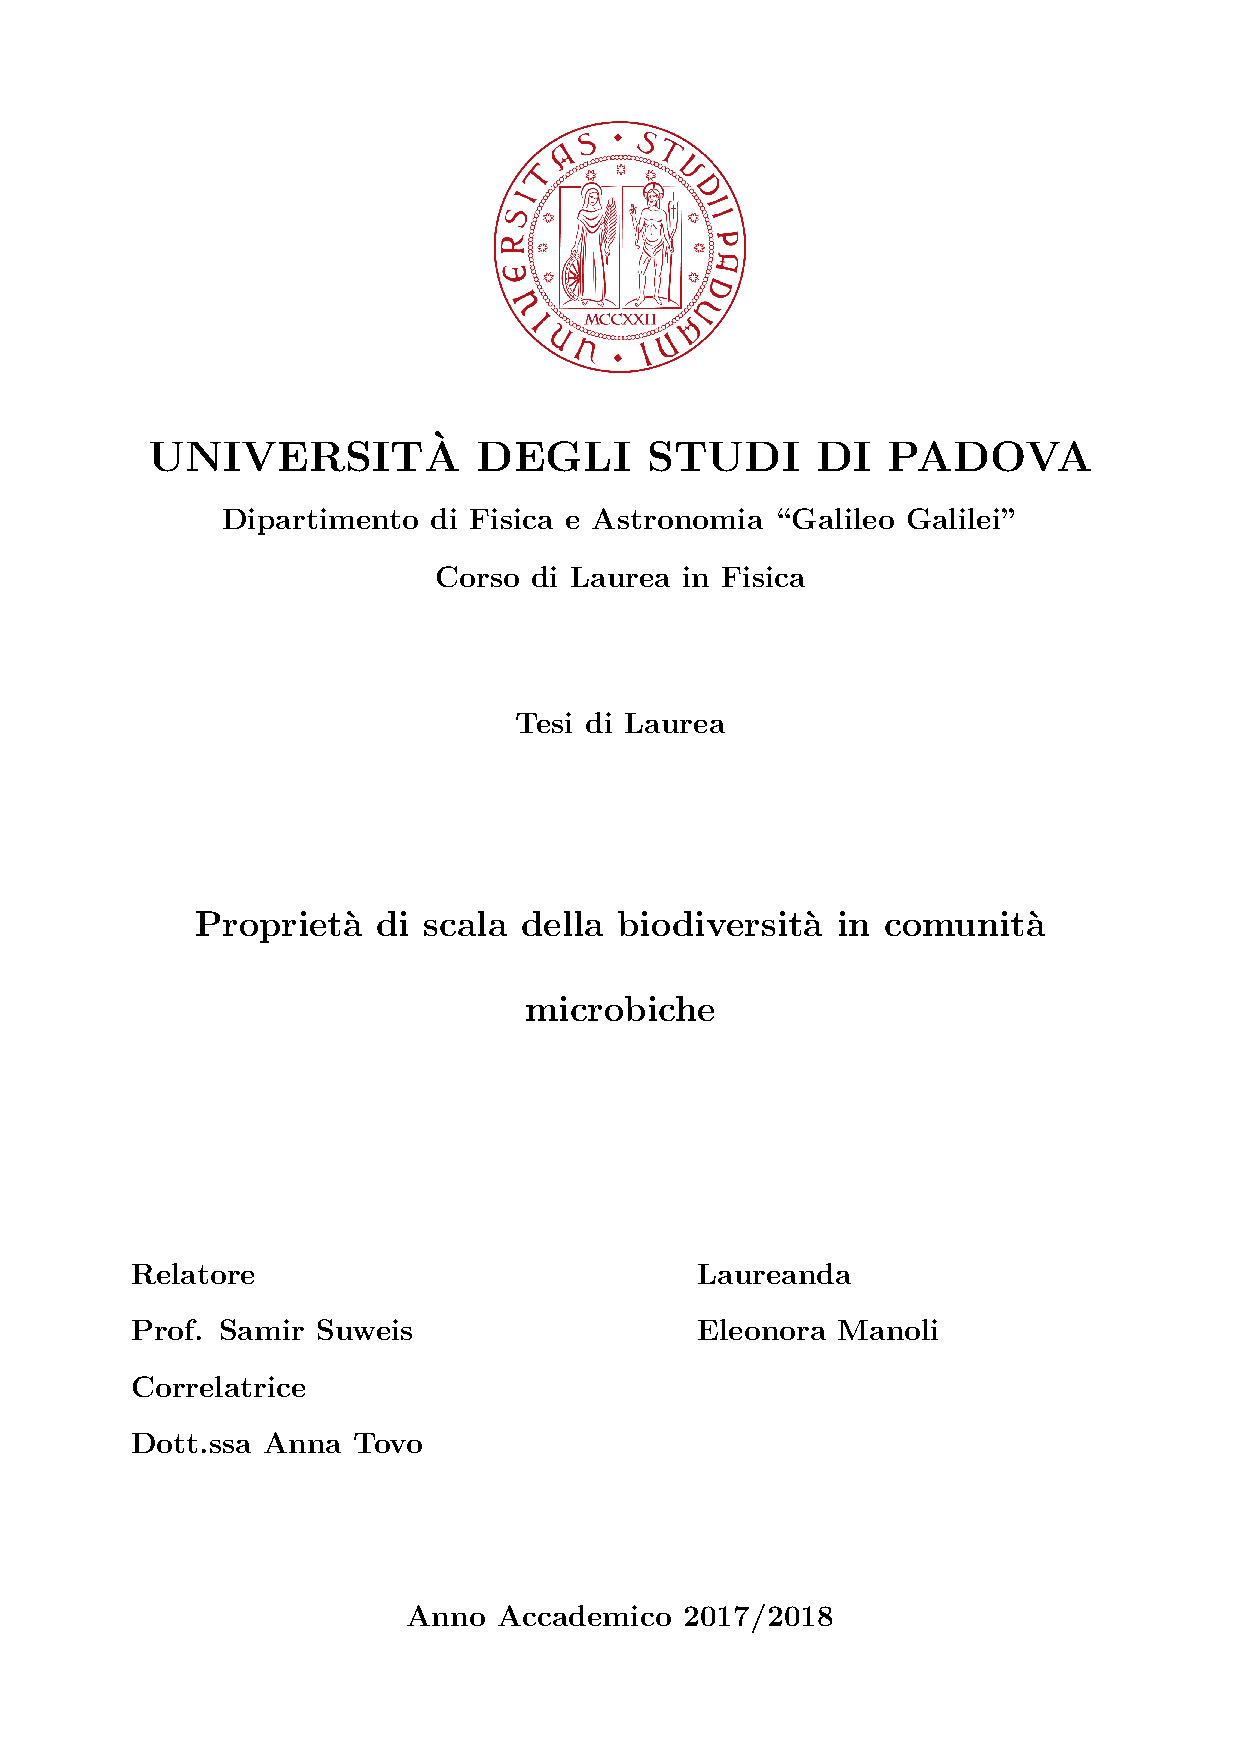
\includepdf{Frontespizio_Laurea.pdf}
\clearpage
\thispagestyle{empty}
\phantom{a}
%\maketitle
\chapter{Abstract}
 

% -------------------------------- TRACCIA GUIDA PER LA STESURA ------------------------------
%Il sommario � un breve riassunto dell'elaborato, orientativamente di circa 200 parole. In
%esso il laureando deve esporre concisamente:
%
%\begin{itemize}
%\item il problema che � stato considerato
%\item come il problema � stato risolto
%\item i principali risultati e il relativo significato.
%\end{itemize}
%
%Il sommario deve essere informativo e non una semplice lista di argomenti svolti; da una
%sua lettura, con una preparazione media sull'argomento, si dovrebbe capire se il lavoro �
%di interesse per chi si accinge a consultare la tesi.


In ecologia, un problema nella caratterizzazione della biodiversità di un ecosistema è quello di stimarla utilizzando solo campioni locali, i quali coprono solamente una minima percentuale dell'area su cui si estende il sistema in esame. In questa tesi, seguendo il lavoro presentato nell'articolo "Upscaling species richness and abundances in tropical forests"\cite{Tovoe1701438}, recentemente pubblicato su Science Advance, verranno presentati alcuni dei metodi più utilizzati per superare tale problema ponendo l'accento su come questi derivino naturalmente da principi primi alla base dei processi biologici. Un problema analogo si presenta anche nello studio delle comunità microbiche.\newline
Dopo aver testato l'affidabilità dei modelli in questo ambito, verranno applicati a dei dati presi dallo studio "Characterization of the gut microbiome using $16S$ or shotgun metagenomics"\cite{shotgun}.

\clearemptydoublepage

% Indice della tesi
\tableofcontents

%\mainmatter

\clearemptydoublepage

\mainmatter

%\chapter*{Introduzione}
\addcontentsline{toc}{chapter}{Introduzione}
Ogni volta che inviamo una e-mail, visitiamo un sito web o chattiamo con qualcuno, i nostri pacchetti attraversano vari router/server che possono controllare i dati inoltrati. Anche se i dati contenuti nei pacchetti sono crittografati, l'IP header rimane comunque visibile, ed � quindi possibile scoprire le identit� del mittente e del destinatario. Intercettando e analizzando i pacchetti, una spia pu� ottenere un numero considerevole di informazioni circa l'identit� dei soggetti della comunicazione, l'applicazione che li ha generati e talvolta il loro contenuto.
I sistemi di anonymous routing, come l'\emph{Onion Routing}\cite{tor}, nascono per garantire la segretezza nelle comunicazioni e l'anonimato delle parti coinvolte.

L'Onion routing � il pi� diffuso sistema di comunicazione anonimo a bassa latenza, permette web browsing, invio di e-mail, messaggistica istantanea e altri servizi. Esso si basa sulla rete \emph{Tor (The Onion Router)}, formata da un gruppo di volontari, che donano la propria banda per permettere agli utenti di aumentare la loro privacy e la loro sicurezza. La rete viene anche utilizzata come strumento per aggirare censure e blocchi imposti dagli ISP e, pi� in generale, il controllo delle comunicazioni da parte dei governi e dei regimi repressivi. Milioni di persone ogni giorno usano Tor per svolgere le loro attivit� quotidiane (come e-mail, Facebook, Twitter) senza il timore di essere monitorati. Per questo in alcuni paesi del mondo, come Cina, Iran, Kazakistan ecc. si tenta di arginare il pi� possibile la diffusione e l'utilizzo di Tor. In altri paesi, come gli Stati Uniti, viene usato dalla Marina Militare per svolgere operazioni di intelligence e dalle forze dell'ordine per controllare siti web, senza lasciare tracce di indirizzi IP governativi. Anche organizzazioni come Wikileaks utilizzano Tor per scambiare informazioni e tutelare i propri informatori. Attualmente, la rete conta circa 7000 router attivi e approssimativamente 2 milioni di client che si collegano ogni giorno \cite{tormetrics}.



%\emph{anonimato}, \emph{non linkabilit�}, \emph{inosservabilit�}.



%\cite{tor}, nascono per garantire segretezza nelle comunicazioni, in particolare cercando di raggiungere degli obiettivi fondamentali:
%\begin{description}
%\item \textbf{Anonimity}, definita come lo stato di non essere identificabili all'interno di un insieme di soggetti.
%\item \textbf{Unlinkability}.
%\item \textbf{Unobservability}.
%\end{description} 

%i client devono potersi scambiare messaggi in totale anonimato, questo significa che essi non devono essere identificabili all'interno di un insieme di soggetti.


%
%\lipsum[1-4]
%wikileaks

%Essa � costruita sopra ad internet...

%Perch� anonimato, blocco dei governi, cos � attacco dos


%non lascia traccia sui server, IP, vedi survey, gestita da volontari, %dati riguardanti utilizzo di tor, grafici

%\section{Perch\`e l'anonimato}

%\section{Blocco da parte dei governi}

\subsubsection{Attacchi DoS}
L'acronimo \emph{DoS}, abbreviazione di \emph{denial of service}, letteralmente negazione del servizio, indica una tipologia di attacchi informatici che mirano ad esaurire le risorse di un sistema, tipicamente un web server o un router, fino a renderlo non pi� in grado di fornire i propri servizi ai client. Esso non � un attacco caratteristico della rete Tor, dato che, attraverso varie tecniche, pu� essere effettuato contro qualsiasi sistema collegato ad Internet che offre servizi TCP. Quello che � possibile fare, per�, � sfruttare delle debolezze di progettazione del protocollo di Tor per condurre degli attacchi che in una normale rete TCP non sarebbero possibili. Come nei classici attacchi DoS, anche quelli che sfruttano le vulnerabilit� di Tor mirano al consumo di banda, di risorse computazionali o di memoria. Gli attacchi DoS sulle reti di anonimato possono essere suddivisi in due categorie: \emph{blanket blocking}, che blocca l'accesso all'intera rete senza attaccare in modo diretto alcun router, come ad esempio i blocchi imposti dai governi, oppure \emph{targeted attack}, ovvero attacchi con un obiettivo specifico, che tentano di portare nodi della rete offline. Portando offline i router portanti della rete, � possibile, probabilisticamente parlando, deanonimizzare servizi nascosti, scoprire l'identit� di due interlocutori o comunque causare un calo di prestazioni della rete che pu� indurre gli utenti ad utilizzare altri metodi di comunicazione meno sicuri di Tor. 



%Inoltre, molto spesso, vengono utilizzati per scoprire l'identit� di un server o per 

           
%\lipsum[1]

%\chapter{Introduzione}
%L'introduzione costituisce la prima parte dell'elaborato ed estende quanto contenuto nel
%sommario, orientando meglio la lettura. In essa vanno inserite le informazioni che stanno a
%monte, logicamente e cronologicamente, al lavoro svolto nella tesi. Si compone
%essenzialmente dei seguenti punti:
%\begin{itemize}
%\item spiegazione della natura del problema considerato
%\item descrizione dei contenuti reperibili in letteratura relativamente al problema in
%questione, corredata da esaurienti citazioni bibliografiche
%\item scopo del lavoro
%\item indicazione dei metodi di soluzione del problema
%\item elenco schematico del contenuto dei vari capitoli.
%\end{itemize}
%
%\clearemptydoublepage

\chapter*{Introduzione}
\addcontentsline{toc}{chapter}{Introduzione}
Ogni volta che inviamo una e-mail, visitiamo un sito web o chattiamo con qualcuno, i nostri pacchetti attraversano vari router/server che possono controllare i dati inoltrati. Anche se i dati contenuti nei pacchetti sono crittografati, l'IP header rimane comunque visibile, ed � quindi possibile scoprire le identit� del mittente e del destinatario. Intercettando e analizzando i pacchetti, una spia pu� ottenere un numero considerevole di informazioni circa l'identit� dei soggetti della comunicazione, l'applicazione che li ha generati e talvolta il loro contenuto.
I sistemi di anonymous routing, come l'\emph{Onion Routing}\cite{tor}, nascono per garantire la segretezza nelle comunicazioni e l'anonimato delle parti coinvolte.

L'Onion routing � il pi� diffuso sistema di comunicazione anonimo a bassa latenza, permette web browsing, invio di e-mail, messaggistica istantanea e altri servizi. Esso si basa sulla rete \emph{Tor (The Onion Router)}, formata da un gruppo di volontari, che donano la propria banda per permettere agli utenti di aumentare la loro privacy e la loro sicurezza. La rete viene anche utilizzata come strumento per aggirare censure e blocchi imposti dagli ISP e, pi� in generale, il controllo delle comunicazioni da parte dei governi e dei regimi repressivi. Milioni di persone ogni giorno usano Tor per svolgere le loro attivit� quotidiane (come e-mail, Facebook, Twitter) senza il timore di essere monitorati. Per questo in alcuni paesi del mondo, come Cina, Iran, Kazakistan ecc. si tenta di arginare il pi� possibile la diffusione e l'utilizzo di Tor. In altri paesi, come gli Stati Uniti, viene usato dalla Marina Militare per svolgere operazioni di intelligence e dalle forze dell'ordine per controllare siti web, senza lasciare tracce di indirizzi IP governativi. Anche organizzazioni come Wikileaks utilizzano Tor per scambiare informazioni e tutelare i propri informatori. Attualmente, la rete conta circa 7000 router attivi e approssimativamente 2 milioni di client che si collegano ogni giorno \cite{tormetrics}.



%\emph{anonimato}, \emph{non linkabilit�}, \emph{inosservabilit�}.



%\cite{tor}, nascono per garantire segretezza nelle comunicazioni, in particolare cercando di raggiungere degli obiettivi fondamentali:
%\begin{description}
%\item \textbf{Anonimity}, definita come lo stato di non essere identificabili all'interno di un insieme di soggetti.
%\item \textbf{Unlinkability}.
%\item \textbf{Unobservability}.
%\end{description} 

%i client devono potersi scambiare messaggi in totale anonimato, questo significa che essi non devono essere identificabili all'interno di un insieme di soggetti.


%
%\lipsum[1-4]
%wikileaks

%Essa � costruita sopra ad internet...

%Perch� anonimato, blocco dei governi, cos � attacco dos


%non lascia traccia sui server, IP, vedi survey, gestita da volontari, %dati riguardanti utilizzo di tor, grafici

%\section{Perch\`e l'anonimato}

%\section{Blocco da parte dei governi}

\subsubsection{Attacchi DoS}
L'acronimo \emph{DoS}, abbreviazione di \emph{denial of service}, letteralmente negazione del servizio, indica una tipologia di attacchi informatici che mirano ad esaurire le risorse di un sistema, tipicamente un web server o un router, fino a renderlo non pi� in grado di fornire i propri servizi ai client. Esso non � un attacco caratteristico della rete Tor, dato che, attraverso varie tecniche, pu� essere effettuato contro qualsiasi sistema collegato ad Internet che offre servizi TCP. Quello che � possibile fare, per�, � sfruttare delle debolezze di progettazione del protocollo di Tor per condurre degli attacchi che in una normale rete TCP non sarebbero possibili. Come nei classici attacchi DoS, anche quelli che sfruttano le vulnerabilit� di Tor mirano al consumo di banda, di risorse computazionali o di memoria. Gli attacchi DoS sulle reti di anonimato possono essere suddivisi in due categorie: \emph{blanket blocking}, che blocca l'accesso all'intera rete senza attaccare in modo diretto alcun router, come ad esempio i blocchi imposti dai governi, oppure \emph{targeted attack}, ovvero attacchi con un obiettivo specifico, che tentano di portare nodi della rete offline. Portando offline i router portanti della rete, � possibile, probabilisticamente parlando, deanonimizzare servizi nascosti, scoprire l'identit� di due interlocutori o comunque causare un calo di prestazioni della rete che pu� indurre gli utenti ad utilizzare altri metodi di comunicazione meno sicuri di Tor. 



%Inoltre, molto spesso, vengono utilizzati per scoprire l'identit� di un server o per 

           
%\lipsum[1]

%\chapter{Introduzione}
%L'introduzione costituisce la prima parte dell'elaborato ed estende quanto contenuto nel
%sommario, orientando meglio la lettura. In essa vanno inserite le informazioni che stanno a
%monte, logicamente e cronologicamente, al lavoro svolto nella tesi. Si compone
%essenzialmente dei seguenti punti:
%\begin{itemize}
%\item spiegazione della natura del problema considerato
%\item descrizione dei contenuti reperibili in letteratura relativamente al problema in
%questione, corredata da esaurienti citazioni bibliografiche
%\item scopo del lavoro
%\item indicazione dei metodi di soluzione del problema
%\item elenco schematico del contenuto dei vari capitoli.
%\end{itemize}

\clearemptydoublepage

\chapter{Master Equation}
In questo capitolo vediamo come si possono ricavare la distribuzione binomiale negativa e la Log Series modellizzando la dinamica dell'abbondanza delle specie attraverso un'equazione che descrive la nascita e la morte degli individui : la \emph{birth-death master equation}.

\section{Distribuzione binomiale negativa}
%La distribuzione binomiale negativa può essere derivata dai principi primi alla base dei processi biologici: sia $\emph{P}_{\emph{n,s}}(t)$ la probabilità che ad un certo tempo t, la specie \emph{s} abbia esattamente \emph{n} individui, con \emph{s}\in$\left \{ 1,...,S \right \}$. Assumiamo che la dinamica della popolazione di ogni specie sia governata da due termini: i rate di nascita e di morte, rispettivamente, $\emph{b}_\emph{{n,s}}$ e $\emph{d}_\emph{{n,s}}$, per una specie \emph{s} con \emph{n} individui.
L'equazione che regola l'evoluzione di $\emph{P}_{\emph{n,s}}(t)$ per $\emph{n}\ge0$ è la seguente:
\begin{equation}
\frac{\partial\emph{P}_{\emph{n,s}}(t)}{\partial\emph{t}}=
\emph{P}_{\emph{n-1,s}}(t)\emph{b}_\emph{{n-1,s}}+\emph{P}_{\emph{n+1,s}}(t)\emph{d}_\emph{{n+1,s}}-\emph{P}_{\emph{n,s}}(t)\emph{b}_\emph{{n,s}}-\emph{P}_{\emph{n,s}}(t)\emph{d}_\emph{{n,s}}.
\label{eq:master}
\end{equation}
Imponendo condizioni al contorno riflettenti, $\emph{b}_\emph{{-1,s}}=\emph{d}_\emph{{0,s}}=0$, la (\ref{eq:master}) è valida anche per $\emph{n}=0$ e \emph{n=1}. Per $n>0$ la soluzione stazionaria è:
\begin{equation}
\emph{P}_{\emph{n,s}}=P_{0,\emph{s}}\prod_{i=0}^{n-1}\frac{\emph{b}_\emph{{i,s}}}{\emph{d}_\emph{{i+1,s}}}
\label{eq:steadystate}
\end{equation}
dove il termine $P_{0,\emph{s}}$ è il fattore di normalizzazione che può essere trovato imponendo la condizione $\sum_{n=1}^\infty \emph{P}_{\emph{n,s}}=1.$ Notiamo che la somma inizia da \emph{n}=1 in quanto non si considerano specie con abbondanza nulla.\\
Assumiamo ora che $\emph{b}_\emph{{n,s}}$ dipenda da un termine indipendente dal numero di individui $\emph{b}_\emph{s}$, cioè il tasso di nascita pro capite, e dal termine $\emph{r}_\emph{s}$, che tiene conto di eventi di immigrazione o di interazioni intraspecifiche:
\begin{equation}
\emph{b}_\emph{n,s}=\emph{b}_\emph{s}(n+\emph{r}_\emph{s}).
\label{eq:birthNB}
\end{equation}
Analogamente assumiamo che il termine $\emph{d}_\emph{n,s}$ dipenda da $\emph{d}_\emph{s}$, cioè dal tasso di morte pro capite:
\begin{equation}
\emph{d}_\emph{n,s}=\emph{d}_\emph{s}\emph{n}.
\label{eq:deathNB}
\end{equation}
Queste supposizioni sono ragionevoli in ecologia.\\
Sostituendo questi ultimi termini nella (\ref{eq:steadystate}) e denotando con $\xi_\emph{s}=\emph{b}_\emph{s}/\emph{d}_\emph{s}$, si ottiene:
$$
\emph{P}_\emph{n,s}=P_\emph{0,s}\binom{n+\emph{r}_\emph{s}-1}{n}\xi_\emph{s}^n.
$$
La costante di normalizzazione può essere calcolata imponendo:
$$
1=\sum_{n=1}^\infty \emph{P}_{\emph{n,s}}=P_\emph{0,s}\sum_{n=0}^\infty\binom{n+\emph{r}_\emph{s}-1}{n}\xi_\emph{s}^n=P_\emph{0,s}[1-(1-\xi_\emph{s})^{\emph{r}_\emph{s}}](1-\xi_\emph{s})^{-\emph{r}_\emph{s}}
$$
Dunque la probabilità che una specie \emph{s} abbia \emph{s} individui all'equilibrio è data da una binomiale negativa di parametri $(\emph{r}_\emph{s}, \xi_\emph{s})$ e normalizzata per abbondanze non nulle ($n\ge 1$):
\begin{equation}
\emph{P}_\emph{n,s}^{\emph{NB}}=\frac{1}{1-(1-\xi_\emph{s})^{\emph{r}_\emph{s}}}\binom{n+\emph{r}_\emph{s}-1}{n}\xi_\emph{s}^n(1-\xi_\emph{s})^{\emph{r}_\emph{s}}.
\label{eq:NBprobability}
\end{equation}
Sotto l'ipotesi della teoria neutrale,secondo la quale le specie sono considerate demograficamente equivalenti(cioè ogni individuo ha la stessa probabilità di procreare,morire e migrare), possiamo rimuovere l'indice \emph{s} di specie dall'equazione sopra, ottenendo così una RSA per l'ecosistema in esame.

\section{La distribuzione logaritmica di Fisher}
Notiamo che,scegliendo in modo diverso i termini $\emph{b}_\emph{n,s}$ e $\emph{d}_\emph{n,s}$,si può ottenere,partendo dalla \emph{birth death master equation} (\ref{eq:master}), un'altra importante distribuzione: la Fisher Log Series.
Assumiamo che la dinamica della popolazione di una comunità sia governata dal corso ecologico e dalla speciazione casuale invece che dalla migrazione da comunità esterne (?).
Allora possiamo porre:
\begin{equation}
    \emph{b}_\emph{n,s}=\emph{b}_\emph{s}n+\delta_\emph{n,0}\nu
\label{eq:birthlog}
\end{equation}
Aggiungendo la condizione al contorno riflettente $\emph{b}_\emph{0,s}=\nu$ si ha che il tasso di nascita tiene conto della riproduzione e della speciazione. In particolare, il parametro $\nu$ assicura che, se le specie si estinguono, la comunità rimane sempre popolata da un individuo.
Dunque sostituendo la (\ref{eq:deathNB}) e la (\ref{eq:birthlog}) nella (\ref{eq:steadystate}) e definendo $\emph{x}_emph{s}=\emph{b}_\emph{s}/\emph{d}_\emph{s}$, si trova la seguente soluzione stazionaria:
\begin{equation}
    \emph{P}_\emph{n,s}=P_\emph{0,s}\frac{\nu}{\emph{b}_\emph{s}}\frac{\emph{x}_\emph{s}^{\emph{n}}}{\emph{n}}.
\end{equation}
La costante di normalizzazione $P_\emph{0,s}$ si determina imponendo:
$$
1=\sum_{n=1}^\infty \emph{P}_{\emph{n,s}}=P_\emph{0,s}\frac{\nu}{\emph{b}_\emph{s}}\sum_{n=0}^\infty\frac{\emph{x}_\emph{s}^{\emph{n}}}{\emph{n}}=P_\emph{0,s}\frac{\nu}{\emph{b}_\emph{s}}[-\log(1-\emph{x}_\emph{s})].
$$
Dunque abbiamo:
%\begin{equation}
%    \emph{P}_\emph{n,s}^{\emp{LS}}=-\frac{1}{\log(1-\emph{x}_\emph{s})}\frac{\emph{x}_\emph{s}^{\emph{n}}}{\emph{n}}.
%\label{eq:fisherdist}
%\end{equation}
Anche in questo caso assumiamo che le specie siano equivalenti e possiamo dunuq omettere l'indice \emph{s}.

\subsection{La distribuzione di Fisher come caso particolare della binomiale negativa}
Osserviamo che la distribuzione binomiale negativa converge ad una distribuzione logarimtica nel limite di \emph{r} che tende a zero:
\begin{equation}
    \lim_{\emph{r} \to 0}\emph{P}_\emph{n}^{\emph{NB}}= \lim_{\emph{r}\to0}\frac{(1-\xi)^{\emph{r}}}{1-(1-\xi)^{\emph{r}}}\binom{n+\emph{r}-1}{n}\xi^n=\frac{\xi^n}{-n\ln(1-\xi)},
\label{eq:convergence}
\end{equation}
dove si è usato il fatto che:
$$
\binom{n+\emph{r}-1}{n}=\frac{\Gamma(\emph{n}+\emph{r})}{\Gamma(\emph{n+1}\Gamma(\emph{r}))} \approx\frac{\emph{r}}{\emph{n+1}},
$$
per $\emph{r}\approx 0$.\\
Notiamo dunque che la (\ref{eq:convergence}) coincide con la (\ref{eq:fisherdist}) ponendo  $\emph{x}=\xi$.


%\section{Protocolli crittografici}
%HTTPS, TLS, Diffie-Hellman, SHA-1
% ---- ELEMENTI UTILI E GIA' PRONTI! ----
%Secondo capitolo della tesi. Esempio di citazione doppia \cite{Munoz-Lipo,Vas}.

%Esempio di figura in \figurename\ \ref{FIG:LogoUniPD}.
%
%\begin{figure}[!htbp]
%\centering
%
\includegraphics[width=0.25\textwidth]{./figure//LogoUniPD}
%\caption{Esempio di figura.}
%\label{FIG:LogoUniPD}
%\end{figure}
%
%Esempio di tabella in \tablename\ \ref{TAB:Esempio}.
%
%\begin{table}[!htbp]
%\centering
%\renewcommand{\arraystretch}{1.3}
%\caption{Esempio di tabella.}
%\begin{tabular}{cc}
%\hline
%Nome & Valore \\
%\hline
%a & 1 \\
%b & 2 \\
%c & 3 \\
%d & 4 \\
%e & 5 \\
%f & 6 \\
%\hline
%\end{tabular}
%\label{TAB:Esempio}
%\end{table}

\clearemptydoublepage

\chapter{Il metodo di upscaling}
In questa sezione vediamo come è possibile ricostruire la biodiversità di un intero ecosistema a partire da un campione ridotto di SAD. \\

....
%(spiegare che il modello nasce in ambito ecologico)\\
%(come viene fatto il campionamento)\\
%(parlare in generale, numero di singleton, specie rare)\\
%(metodo di Chao??)\\
\\
\section{Metodo della binomiale negativa}
Il quadro analitico all'interno del quale si svolge questo lavoro è bastato sui seguenti passaggi:
\begin{itemize}
    \item Campionare una frazione $\emph{p}^*$ dell'intera foresta e ottenere il vettore delle abbondanze delle $S^*$ specie campionate, $\emph{n}_{\emph{p}^*}={\emph{n}_1,\emph{n}_2,...,\emph{n}_{S^*}}$
    \item Usare una combinazione lineare di binomiali negative con lo stesso $\hat \xi_{\emph{p}^*}$ e diversi valori di \emph{r} per fittare la SAD sperimentale al desiderato grado di accuratezza.
\end{itemize}
Di seguito analizzeremo in dettaglio il metodo,le proprietà e i passaggi che ci permettono di ottenere le informazioni desiderate.\\
Quando facciamo upscaling siamo interessati alla SAD ed al numero totale di specie presenti a scala totale,cioè in tutta l'area della foresta\emph{A}.
Denotiamo con P(\emph{n}|1) la probabilità che una specie abbia esattamente \emph{n} individui a scala totale(qui con il numero 1 si denota l'intera foresta), anche nota come \emph{abbondanza relativa delle specie} RSA.
Notiamo che P(\emph{n}|1) deve essere definita solamente per $\emph{n}\ge1$ poiché, a scala totale, una data specie deve avere almeno un individuo.
In questo contesto si ipotizza che la SAD segua una distribuzione binomiale negativa, \emph{P}(\emph{n}|\emph{r},$\xi$) di parametri (\emph{r},$\xi$):
\begin{equation}
 P(\emph{n}|1)=\emph{c}(\emph{r},\xi)\emph{P}(\emph{n}|\emph{r},\xi)
 \label{eq:NBfunctform}
\end{equation}
\\
con 
\begin{equation}
    \emph{P}_\emph{n}=\binom{n+\emph{r}-1}{n}\xi^n(1-\xi)^{\emph{r}},      
    \emph{c}(\emph{r}\xi)=\frac{1}{1-(1-\xi)^{\emph{r}}}
\end{equation}
dove \emph{c} è la costante di normalizzazione.
Quest'ultima è stata calcolata imponendo $\sum_{\emph{n}=1}^\infty P(\emph{n}|1)$, dove la somma parte da 1 poiché le specie con abbondanza nulla a scala totale saranno assenti anche a scale ridotte.
Notiamo che \emph{p}(\emph{n}|\emph{r},$\xi$) è normalizzata per $\emph{n}\ge0$: questo perché, nei sotto campioni, esiste una probabilità non nulla di trovare una specie, presente nell'intera foresta, avente \emph{n}=0 individui.In questo modo si tiene conto del numero di specie mancanti nei sotto campioni.\\
Consideriamo ora un campione di foresta di area \emph{a} e definiamo \emph{p}=\emph{a}/\emph{A} la scala del campione, cioè la frazione di foresta osservata.
Come primo passaggio calcoliamo la RSA del campione assumendo che quest'ultima non sia influenzata da correlazioni spaziali. Quest'ipotesi è ben soddisfatta ed è stata verificata usando dati di foreste generati \emph{in silico} a vari gradi di correlazione spaziale.(citare qualcosa, ci devo tornare sopra??)\\
Sotto queste ipotesi la probabilità che una specie presenti \emph{k} individui in un'area \emph{a=pA}, condizionata dal fatto che presenta \emph{n} individui nella regione totale \emph{A} è data dalla distribuzione binomiale:
\begin{equation}
\emph{P}_\emph{binom}(\emph{k|p,n})=\begin{cases} \binom{\emph{n}}{\emph{k}}\emph{p}^\emph{k}(1-\emph{p})^{\emph{n-k}}, & \mbox{se }\emph{k}=0,...,\emph{n} \\ 0, & \mbox{se }n\mbox{\emph{k>n}}
\end{cases}
\end{equation}

Infatti,in assenza di correlazioni spaziali, la probabilità che uno degli individui di una specie si trovi in una regione di area \emph{a} è esattamente \emph{p}.(?controllare?)

Mostriamo ora un risultato chiave per il metodo di upscaling:
\subsection{Proprietà di auto-somiglianza della distribuzione binomiale negativa}
Sia P(\emph{n}|1)=\emph{c}(\emph{r},$\xi$)\emph{P}(\emph{n}|\emph{r},$\xi$) la RSA della foresta a scala totale e denotiamo con \emph{P}(\emph{k}|\emph{r},$\xi$) la probabilità che una specie abbia abbondanza \emph{k} alla scala \emph{p}$\in$(0,1), condizionata dal fatto che alla scala totale \emph{A} sono presenti \emph{n} individui di quella specie.
Se \emph{P}(\emph{k}|\emph{n,p})=$\emph{P}_\emph{binom}(\emph{n}|\emph{r},\xi)$ segue una distribuzione binomiale, allora la RSA $\emph{P}_\emph{sub}(\emph{k}|\emph{p})$ alla scala di campionamento \emph{p} è ancora una binomiale negativa per $\emph{k}\ge1$ con il parametro $\xi$ riscalato e lo stesso \emph{r}:
\begin{equation}
    \emph{P}_\emph{sub}(\emph{k}|\emph{p})=\begin{cases} \emph{c}(\emph{r},\xi)\emph{P}(\emph{k}|\emph{r},\xi), & \mbox{ }\emph{k}\ge1 \\ 1-\emph{c}(\emph{r},\xi)/\emph{c}(\emph{r},\hat\xi_{\emph{p}}), & \mbox{ }\mbox{\emph{k=0}}
    \end{cases}
\label{eq:RSAbinom}
\end{equation}

con 
\begin{equation}
    \hat\xi_{\emph{p}}=\frac{\emph{p}\xi}{1-\xi(1-\emph{p})}
\label{eq:NBparametersub}
\end{equation}

DIMOSTRAZIONE?\\
\\
Ricordiamo che questo metodo fa uso solamente delle informazioni che si possono ottenere da un campione ad una certa scala $p^*$, infatti noi abbiamo informazioni solo sulle abbondanze delle $S^*\le S$ specie presenti nel campione esaminato. Denotando il numero di specie di abbondanza \emph{k} alla scala $p^*$ con $S^*(\emph{k})$, otteniamo, per $\emph{k}\ge 1$:
\begin{equation}
    \frac{S^*(\emph{k})}{S^*}\equiv P(\emph{k}|\emph{p}^*)=\frac{\emph{P}_\emph{sub}(\emph{k}|\emph{p}^*)}{\sum_{k^{'} \ge 1}^{} \emph{P}_\emph{sub}(\emph{k}^{'}|\emph{p}^{*})}
    =\frac{\emph{P}(\emph{k}|\emph{r},\hat\xi_{\emph{p}^*})}{\sum_{k^{'} \ge 1}^{} \emph{P}(\emph{k}^{'}|\emph{r},\hat \xi_{\emph{p}^*})}
    =\emph{c}(\emph{r},\hat\xi_{\emph{p}^*})\emph{P}(\emph{k}|\emph{r},\hat \xi_{\emph{p}^*})
    \label{eq:SstarRSA}
\end{equation}
che, dalla (\ref{eq:NBfunctform}), è una binomiale negativa normalizzata per $\emph{k}\ge 1$, mentre $\emph{P}(\emph{k}|\emph{r},\hat \xi_{\emph{p}^*}$ è normalizzata per $\emph{k}\ge 0$.
Per quanto detto sopra otteniamo dunque il seguente risultato: partendo da una distribuzione binomiale negativa per la RSA a scala globale, anche la RSA a scala ridotta risulta distribuita secondo una binomiale negativa di parametri lo stesso \emph{r} e $\hat \xi_\emph{p}^*$ riscalato.
Una RSA avente la proprietà di avere la stessa forma funzionale a scale differenti è detta essere \emph{invariante per forma}.

\subsection{Il numero di specie a scala totale}
Fittando la RSA dei dati alla scala $\emph{p}^*$ possiamo dunque trovare i parametri \emph{r} e $\hat \xi_\emph{p}^*$ e, invertendo l'equazione (\ref{eq:NBparametersub}), troviamo:
\begin{equation}
    \xi=\frac{\hat \xi_{\emph{p}^*}}{\emph{p}^*+\hat \xi_{\emph{p}^*}(1-\emph{p}^*)}
\label{eq:NBparameter}
\end{equation}
Usando ancora la (\ref{eq:NBparametersub}) per eliminare $\xi$ dall'ultima equazione, otteniamo la seguente relazione per il parametro $\xi$ alle due scale \emph{p} e $\emph{p}^*$:
\begin{equation}
    \hat\xi_\emph{p}=\frac{p \hat \xi_{\emph{p}^*}}{\emph{p}^*+\hat\xi_{\emph{p}^*}(\emph{p}-\emph{p}^*)}\equiv U(\emph{p},\emph{p}^*|\hat \xi_{\emph{p}^*})
    \label{eq:xihatp}
\end{equation}
dalla quale, ovviamente, è possibile riottenere sia la (\ref{eq:NBparametersub}) che la (\ref{eq:NBparameter}) ponendo $\xi \equiv \hat \xi_{\emph{p}=1} $.

Vogliamo ora determinare la relazione tra il numero totale di specie S alla scala totale \emph{p}=1 e il numero totale di specie osservate localmente $S_\emph{p}$ alla scala \emph{p}.
D'ora in avanti per denotare il numero di specie alla scala locale useremo la notazione $S^*\equiv S_{\emph{p}^*}$.
Notiamo che:
\begin{equation}
\emph{P}_\emph{sub}(\emph{k=0}|\emph{p}^*)=\frac{S-S^*}{S}
\end{equation}
\begin{equation}
    \emph{P}_\emph{sub}(\emph{k=0}|\emph{p}^*)=\frac{S^*(\emph{k})}{S}.
\end{equation}
Usando la seconda delle (\ref{eq:RSAbinom}), il numero di specie presenti nell'intera foresta è dato, in termini dei dati del campione osservato, da:
\begin{equation}
S=\frac{S^*}{1-\emph{P}_\emph{sub}(\emph{k}=0|\emph{p}^*)}=S^*\frac{1-(1-\xi)^r}{1-(1-\hat \xi_{\emph{p}}^*)^r}
\label{eq:upscaleNB}
\end{equation}

Notiamo che, se si assume che la RSA segua una distribuzione binomiale negativa a scala globale, il valor medio dell'abbondanza totale riscala linearmente con l'area, infatti:
(AGGIUNGERE EQ S26)

\section{Metodo della distribuzione di Fisher}
Ora mostreremo che è possibile risalire al numero di specie anche quando si suppone che la SAD a scala globale sia distribuita secondo una log-series.\\
Supponiamo che la RSA a scala globale sia distribuita secondo una distribuzione logaritmica con parametro \emph{x}:

\begin{equation}
P(\emph{n}|1)=P^{\emph{LS}}(\emph{n}|\emph{x})=\alpha(x)\frac{\emph{x}^\emph{n}}{\emph{n}}, \alpha(x)=-(\log(1-\emph{x}))^{-1}
\end{equation}
dove $\alpha(x)$ è la costante di normalizzazione.
Assumendo anche questa volta che la RSA del campione non sia affetta da correlazioni spaziali si trova che anche la log-series soddisfa la proprietà di auto somiglianza.

\subsection{Proprietà di auto-somiglianza della distribuzione logaritmica di Fisher}
Sia $P(\emph{n}|1)=\alpha(\emph{x})\emph{P}^{\emph{LS}}(\emph{n}|\emph{x})$ la RSA alla scala globale e denotiamo con $\emph{P}(\emph{k})|\emph{n,p}$ la probabilità che una specie abbia abbondanza \emph{k} nel campione alla scala \emph{p} $\in$ (0,1) condizionata dal fatto  alla scala totale \emph{A} la specie possiede \emph{n} individui.\\
Se \emph{P}(\emph{k}|\emph{n,p})=$\emph{P}_\emph{binom}(\emph{k}|\emph{n,p})$ è distribuita secondo una binomiale, allora la RSA alla scala del campione, $\emph{P}^\emph{LS}_\emph{sub}(\emph{k}|\emph{p})$, è ancora una log-series per $\emph{k}\ge 1$ con il parametro \emph{x} riscalato:

\begin{equation}
\emph{P}^\emph{LS}_\emph{sub}(\emph{k}|\emph{p})=\begin{cases} n/2, & \mbox{se }n\mbox{ pari} \\ 3n+1, & \mbox{se }n\mbox{ dispari}
\end{cases}
\end{equation}
con



\begin{equation}
\emph{$\hat x$}_\emph{p}=\frac{\emph{px}}{1-\emph{x}(1-\emph{p})}
\label{eq:LSparametersub}
\end{equation}
DIMOSTRAZIONE??

Notiamo che (\ref{eq:LSparametersub}) è analoga a (\ref{eq:NBparametersub}). Dunque l'analogo di (\ref{eq:NBparameter}) è


\begin{equation}
\emph{x}=\frac{\emph{$\hat x$}_\emph{p}}{\emph{p}+\emph{$\hat x$}_\emph{p}(1-\emph{p})}
\label{eq:LSparameter}
\end{equation}

e l'equazione (\ref{eq:xihatp}) vale anche in questo caso.


La RSA può essere ottenuta come nell'equazione (\ref{eq:SstarRSA}) ed è data da:

\begin{equation}
P(\emph{k}|\emph{p})=\frac{\emph{P}^\emph{LS}_\emph{sub}}{\sum_{k^{'} \ge 1}^{} \emph{P}^\emph{LS}_\emph{sub}(\emph{k}^{'}|\emph{p})}=\alpha(\emph{$\hat x$}_\emph{p}) \frac{\emph{$\hat x$}^\emph{k}_\emph{p}}{\emph{k}}=P^\emph{LS}(\emph{n}| \emph{$\hat x$}_\emph{p})
\end{equation}

Poiché la distribuzione logaritmica di Fisher è un caso particolare della binomiale negativa, è anch'essa invariante per scala.


\subsection{Il numero di specie a scala totale}
Il numero di specie con popolazione $\emph{k} \ge 1$ presenti nel sotto-campione di area \emph{a}=\emph{pA} è dato da:

\begin{equation}
S_\emph{p}(k) \equiv S\emph{P}_\emph{sub}(\emph{k}|\emph{p})=S\alpha(\emph{x})\frac{\emph{$\hat x$}^\emph{k}_\emph{p}}{\emph{k}}=\hat \alpha \frac{\emph{$\hat x$}^\emph{k}_\emph{p}}{\emph{k}}
\end{equation} 
dove abbiamo unito le costanti S e $\alpha (\emph{x})$ in un unico termine $\hat \alpha$ che non dipende dalla scala \emph{p} del campione. Quando ci riferiremo alla scala $\emph{p}^*$ useremo, per brevità di notazione, $S^*(\emph{k})\equiv S_{\emph{p}^*}(\emph{k})$.\\
Allora il numero totale di specie $S^*$ e l'abbondanza totale $N^*$ (?) alla scala $\emph{p}^*$ sono date rispettivamente da:

\begin{equation}
S^*=\sum_{\emph{k}=1}^\infty S^*(\emph{k})=-\hat \alpha \log (1-\emph{$\hat x$}_{\emph{p}^*})
\label{eq:SstarLS}
\end{equation}

\begin{equation}
N^*=\emph{k}\sum_{\emph{k}=1}^\infty S^*(\emph{k})=\hat \alpha \frac{\emph{$\hat x$}_{\emph{p}^*}}{1-\emph{$\hat x$}_{\emph{p}^*}}
\label{eq:NstarLS}
\end{equation}

Poiché $S^*$ e $N^*$ sono note dal campione, possiamo trovare $\hat \alpha$ risolvendo la seguente equazione:

\begin{equation}
N^*- \hat \alpha(\exp( \frac{S^*}{\hat \alpha})-1)=0
\label{eq:solve}
\end{equation}

che è si ottiene inserendo l'espressione di $  \emph{$\hat x$}_{\emph{p}^*} $ da (\ref{eq:SstarLS}) nella (\ref{eq:NstarLS}).

Vogliamo ora dedurre le informazioni a scala globale \emph{p}=1 dai dati disponibili alla scala \emph{p}=$\emph{p}^*$. Dalle considerazioni precedenti sappiamo che $ \hat \alpha$ è un parametro indipendente dalla scala, dunque abbiamo le seguenti relazioni per S e N:

\begin{equation}
S=-\hat \alpha \log(1-\emph{x})
\label{eq:SLS}
\end{equation}

\begin{equation}
N=\hat \alpha \frac{\emph{x}}{1-\emph{x}}
\label{eq:NLS}
\end{equation}

dalle quali otteniamo:

\begin{equation}
S=\hat \alpha \log(1+ \frac{N}{\hat \alpha}),  \hat \alpha=S\alpha(\emph{x}).
\label{eq:SalphaLS}
\end{equation}

Dunque per dedurre la biodiversità a scala globale, S, è necessaria una stima dell'abbondanza totale N. Prendiamo N=$N^*/ \emph{p}^*$. Notiamo che questo è consistente con il nostro quadro teorico nel quale assumiamo che la RSA sia "form-invariant(?)": infatti si può dimostrare che, se si assume che la RSA segua una distribuzione di Fisher a scala globale, il valor medio dell'abbondanza totale riscala linearmente con l'area:

\begin{equation}
\mathbb{E}(N^*)=\sum_{\emph{k}=1}^\infty \emph{k}S^*(\emph{k})=\sum_{\emph{k}=1}^\infty \emph{k} \hat \alpha  \frac{\hat {\emph{x}}^\emph{k}_{\emph{p}^*}}{\emph{k}}=\alpha \frac{\hat {\emph{x}}_{\emph{p}^*}}{1-\hat {\emph{x}}_{\emph{p}^*}}= \hat 	\alpha \frac{\emph{px}}{1-x}= \emph{p}^* \mathbb{E}(N),
\end{equation}

dove abbiamo usato la  (\ref{eq:LSparametersub}).


% ---------------------  ESEMPI UTILI PRONTI ALL'USO  ----------------------------
%TERZO capitolo della tesi. Esempio di citazione doppia \cite{Munoz-Lipo,Vas}.
%
%Esempio di figura in \figurename\ \ref{FIG:LogoUniPD}.
%
%\begin{figure}[!htbp]
%\centering
%
\includegraphics[width=0.25\textwidth]{./figure//LogoUniPD}
%\caption{Esempio di figura.}
%\label{FIG:LogoUniPD}
%\end{figure}
%
%Esempio di tabella in \tablename\ \ref{TAB:Esempio}.
%
%\begin{table}[!htbp]
%\centering
%\renewcommand{\arraystretch}{1.3}
%\caption{Esempio di tabella.}
%\begin{tabular}{cc}
%\hline
%Nome & Valore \\
%\hline
%a & 1 \\
%b & 2 \\
%c & 3 \\
%d & 4 \\
%e & 5 \\
%f & 6 \\
%\hline
%\end{tabular}
%\label{TAB:Esempio}
%\end{table}

\clearemptydoublepage

%\include{./3-/}

\clearemptydoublepage


\clearemptydoublepage

\phantomsection
%\addcontentsline{toc}{chapter}{Considerazioni finali}
\chapter{Conclusioni}


%------------------------------------------------------------------------------------
%Le conclusioni devono essere brevi e comporsi dei seguenti punti:
%\begin{itemize}
%\item indicazione di ci� che si � esposto e del suo significato
%\item analisi comparativa e commento critico dei risultati presentati
%\item spiegazione motivata delle parti omesse o non approfondite
%\item indicazione dei possibili ulteriori sviluppi.
%\end{itemize}
%------------------------------------------------------------------------------------


% ---------------------  ESEMPI UTILI PRONTI ALL'USO  ----------------------------
%TERZO capitolo della tesi. Esempio di citazione doppia \cite{Munoz-Lipo,Vas}.
%
%Esempio di figura in \figurename\ \ref{FIG:LogoUniPD}.
%
%\begin{figure}[!htbp]
%\centering
%
\includegraphics[width=0.25\textwidth]{./figure//LogoUniPD}
%\caption{Esempio di figura.}
%\label{FIG:LogoUniPD}
%\end{figure}
%
%Esempio di tabella in \tablename\ \ref{TAB:Esempio}.
%
%\begin{table}[!htbp]
%\centering
%\renewcommand{\arraystretch}{1.3}
%\caption{Esempio di tabella.}
%\begin{tabular}{cc}
%\hline
%Nome & Valore \\
%\hline
%a & 1 \\
%b & 2 \\
%c & 3 \\
%d & 4 \\
%e & 5 \\
%f & 6 \\
%\hline
%\end{tabular}
%\label{TAB:Esempio}
%\end{table}

%\backmatter

\clearemptydoublepage

%\phantomsection
\addcontentsline{toc}{chapter}{Ringraziamenti}
\chapter*{Ringraziamenti}

Eventuali ringraziamenti personali. % non obbligatorio
%\clearemptydoublepage

\bibliographystyle{IEEEtran}
%\bibliography{IEEEabrv,./7-Bibliografia/Biblio}

\begin{thebibliography}{9} 

\bibitem{tor} R. Dingledine, N. Mathewson, and P. Syverson,\textit{"TOR: The second-generation onion router,"} In USENIX Security Symposium (San Diego, CA, 2004), USENIX Association, pp. 303-320.

\bibitem{tormetrics} Tor Metrics \url{https://metrics.torproject.org/}, [Accesso: 13 Settembre 2016].

\bibitem{torspec} Tor's protocol specifications \url{https://gitweb.torproject.org/torspec.git/tree/dir-spec.txt}, [Accesso: 13 Settembre 2016].

\bibitem{torbridge} Z. Ling, J. Luo, W. Yu, M. Yang, and X. Fu,\textit{"Extensive analysis and large-scale empirical evaluation of Tor bridge discovery,"} in Proc. IEEE INFOCOM, 2012, pp. 2381-2389.

\bibitem{gfc} P. Winter, S. Lindskog, \textit{"How the Great Firewall of China is Blocking Tor,"} Free and Open Communications on the Internet, 2012.

\bibitem{meek} The Tor Project. Meek \url{https://trac.torproject.org/projects/tor/wiki/doc/meek}, [Accesso: 13 Settembre 2016].

\bibitem{domainfronting} D. Fifield, C. Lan, R. Hynes, P. Wegmann, and V. Paxson, \textit{"Blocking-resistant communication through domain fronting,"} Proceedings on Privacy Enhancing Technologies 2015, pp. 1-19.

\bibitem{cellflood} M. V. Barbera, V. P. Kemerlis, V. Pappas, and A. Keromytis, \textit{"CellFlood: Attacking Tor Onion Routers on the Cheap,"} in Proc. ESORICS, Sep. 2013, pp. 664-681.

\bibitem{sniper} R. Jansen, F. Tschorsch, A. Johnson, and B. Scheuermann, \textit{"The sniper attack: Anonymously deanonymizing and disabling the Tor network,"} in Proc. 21st Annu, Symp. NDSS, Feb. 2014, pp. 1-15.

\bibitem{packetspinning} V. Pappas, E. Athanasopoulos, S. Ioannidis, and E. P. Markatos,\textit{"Compromising Anonymity Using Packet Spinning,"} in ISC 08, Sep. 2008.

\bibitem{lochidd} Lasse {\O}verlier and Paul Syverson, \textit{"Locating Hidden Servers,"} in Proceedings of the IEEE Security and Privacy Symposium (S\&P), May 2006.

\bibitem{survey} E. Erdin, C. Zachor, and M. H. Gunes, \textit{"How to Find Hidden Users: A Survey of Attacks on Anonymity Networks,"}. IEEE Commun. Surv. Tutorials, vol. 17, no. 4, pp. 2296-2316, 2015.

\end{thebibliography}

\appendix

\clearemptydoublepage

%\chapter{(se necessaria)}

Allo scopo di rendere pi� scorrevole la lettura del corpo dell'elaborato, in appendice pu�
essere opportuno riportare:
\begin{itemize}
\item i passaggi matematici non essenziali
\item le dimostrazioni di teoremi
\item le tabelle con i risultati di campagne di misure i cui grafici sono inseriti nel corpo
dell'elaborato
\item i listati dei programmi di calcolo
\item i ``data sheet'' di componenti cui si fa riferimento nel testo principale.
\end{itemize} % non obbligatorio
%\clearemptydoublepage

% Lista delle figure (non obbligatoria)
\listoffigures

\clearemptydoublepage

% Lista delle tabelle (non obbligatoria)
\listoftables

\clearemptydoublepage


% Ridefiniamo l'etichetta per le figure e le tabelle
\renewcommand{\figurename}{Fig.}
\renewcommand{\tablename}{Tab.}
% Ridefiniamo percentuali per inserimento figure nel testo
\renewcommand{\topfraction}{0.85}
\renewcommand{\textfraction}{0.1}
\renewcommand{\floatpagefraction}{0.75}

\end{document}